\section{Resultados}

Conociendo los valores iniciales de la se\~nal limpia, el ruido proporcionado y
habiendo obtenido el resultado luego de aplicar los filtros, resulta muy
sencilla una primera aproximaci\'on a los resultados. La idea del experimento es
intentar que la se\~nal recuperada se parezca lo m\'as posible a la original
(sin ruido).

Fue muy simple, entonces, observar la diferencia entre la se\~nal recuperada y
la original de manera gr\'afica, ya sea a trav\'es de ploteos de se\~nales de 1
\'o 2 dimensiones como de la fuente misma como son las im\'agenes en 2
dimensiones.

Acompa\~nando esto por m\'etodos anal\'iticos como el PSNR (Relaci\'on Se\~nal a
Ruido de Pico) fue posible analizar que filtros resultan mejores que otros y en
que casos es mejor aplicar cada uno.

\subsection{Primeros resultados}

Experimentalmente pudimos observar que el filtro cero es bueno, pero el filtro 
exponencial y el promediador son bastante mejores en todos los casos. 
Para poder obtener un mejor filtrado del ruido, decidimos aplicar primero el 
filtro exponencial y luego el promediador, lo que result\'o en un filtrado muy 
bueno dando resultados muy parecidos a la se\~nal original. 

Los adjetivos utilizados se apoyan tanto en el campo sensorial (en las
im\'agenes y gr\'aficos) como en la medida deL PSNR. 

\subsection{Se\~nales en una dimensi\'on}

\subsubsection{Filtro Cero}

El primer filtro analizado fue el m\'as sencillo de implementar, el filtro cero.
Como mencionamos anteriormente, este filtro utiliza un umbral y env\'ia los
puntos que lo sobrepasan (tanto por arriba como por debajo) a cero.

\begin{figure}
\begin {center}
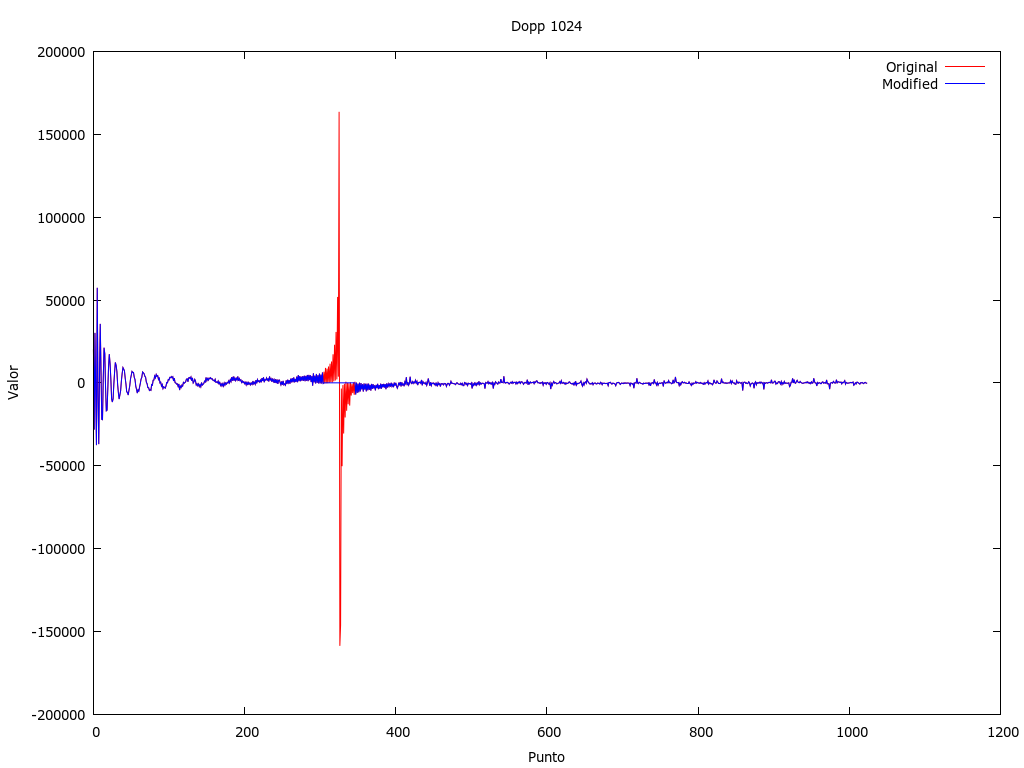
\includegraphics[width=220pt]{../matlab/dopp1024-sin100-zero-spec.png}
\end {center}
\caption{Se\~nal doppler provista por la c\'atedra, transformada, gr\'aficada
luego de aplicar ruido senoidal utilizando el multiplicador 100 (Rojo) y 
habiendo aplicado el filtro cero (azul)}
\label{fig:SinProm}
\end{figure}

Pudimos observar entonces que la se\~nal detecta frecuencias fuera del umbral y
las manda a cero. Este filtro carece de dos caracter\'isticas fundamentales
seg\'un demuestran los experimentos:

\begin{itemize}
	\item {\bf detecci\'on de ``zonas afectadas'':} Como el algoritmo no tiene en
cuenta el contexto a la hora de modificar un punto, la decisi\'on es mandar los
puntos duera del umbral al cero. Esto lleva a ``saltos'' pronunciados en la se\
~nal recuperada.

	\item {\bf elecci\'on de la correspondencia de los puntos fuera del umbral:}
El filtro decide enviar todos los elementos fuera del umbral al cero, con un
manejo de los m\'aximos y minimos globales (en el punto anterior se habla de
locales) se podr\'ia mejorar el resultado del filtro.
\end{itemize}

Sin embargo, como se aprecia en la im\'agen, los resultados son suficientemente
buenos teniendo en cuenta la simplicidad de la implementaci\'on del algoritmo.

\subsubsection{Filtro Exponencial}

\begin{figure}
\begin {center}
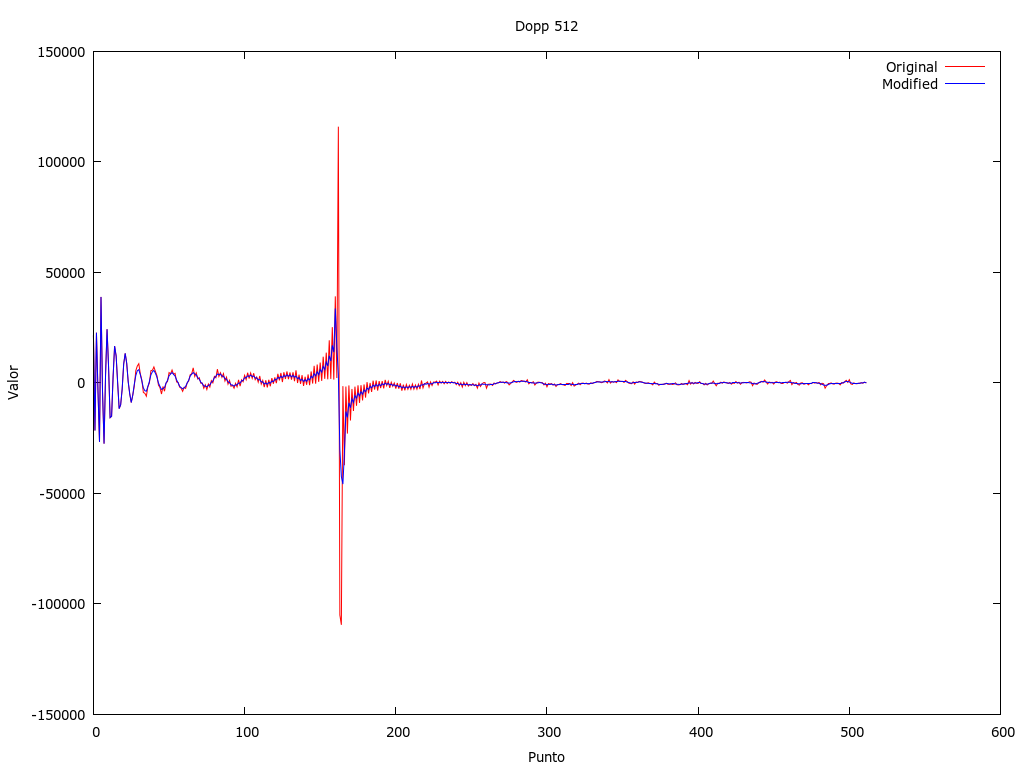
\includegraphics[width=220pt]{../matlab/dopp512-sin100-avg-spec.png}
\end {center}
\caption{Se\~nal doppler provista por la c\'atedra, transformada, gr\'aficada
luego de aplicar ruido senoidal utilizando el multiplicador 100 (Rojo) y 
habiendo aplicado el filtro promedio (azul)}
\label{fig:SinProm}
\end{figure}



\subsection{Se\~nales en dos dimensiones}

